%----------------------------------------------------------------------------------------
%	Hardware
%----------------------------------------------------------------------------------------

\chapter{Hardware Components}

\section{Prior Art}

In this section, existing hardware solutions for digital weighing scales are evaluated. 
The 2nd Gen Xiaomi Smart Scale is an intelligent scale that has the primary function of measuring peoples weights, with many extra functions that allow fitness tracking with connected Xiaomi accounts. It has high precision pressure sensors, and bluetooth connection to the Xiaomi sports app. It shows extra data and suggestions such as fitness plans, but is quite expensive. The Living \& Co Digital Glass Scale is a cheap alternative, with a high precision strain-gauge sensor but only displays the weight through LEDs and does not have any additional functionality. The FitBit Aria Air is a smart scale that functions as a regular weighing scale, but also records weights and synchronises the users biometrics to the FitBit app. This allows users to view trends and data such as their BMI, but like the Xiaomi is quite expensive.

Generally, all physical weight scales are the same, with differences being in the more expensive range having the ability to connect to other devices where weight metrics are processed with other body measurements to give users more information on their health. 




\section{Circuit Topologies}


To detect weight, load cells which contain strain gauges are used. A strain gauge is an electrical sensor that reacts by having an electrical resistance that increases or decreases when weight is applied. The provided load cells have two strain gauges as in Figure \ref{fig:load_cell}. One’s resistance decreases linearly with weight, and the other’s resistance increases linearly. Four load cells are provided, R1, R2, R3, and R4. As such, circuitry is required to connect the load cells and provide one or more output signals from them. 


Topologies to connect the load cells are compared. The load cells could individually be connected to the ADC, as in Figure \ref{fig:sense-1}, allowing weight distribution sensing, however the number of ADC ports provided is insufficient. This option is only possible with an external ADC at additional cost. Another option is connecting all load cells together in a parallel configuration as in Figure \ref{fig:sense-2}. This option is low cost as it requires one processing circuit. However, parallel connections reduce resolution because each load cell's resistance changes are averaged instead of added. Alternatively, a Wheatstone bridge could be used as in Figure \ref{fig:sense-3} to produce a high-resolution output because a Wheatstone bridge adds differences, not averages. Further, this option only requires one processing circuit; thus is a low-cost solution. (Figures B.x are from Appendix B)



Processing the sensed signal is required because the signal is small and to meet requirements of the ADC and chosen op-amp. The requirements are: the signal should be 0 V to 3.3V and an offset to the signal is required for the op-amp. To produce an offset, a Zener regulator or voltage divider with buffer may be used as in Figure \ref{fig:offset}. A Zener regulator output voltage is limited to a few standard values, while the voltage divider output is not. To amplify the signal, an amplifier with double ended inputs must be used, as from a Wheatstone bridge. As such, a differential amplifier as in Figure \ref{fig:amplifier} is suitable. However, its output can vary depending on the load cells' resistances so to prevent this, an instrumentation amplifier is used as in Figure \ref{fig:amplifier-2}.





\section{The Proposed Design}

The proposed design is a Wheatstone bridge and instrumentation amplifier as in Figure \ref{fig:schematic}. The simulated design results are in Figure \ref{fig:simulation}. Values from practical testing were used for the load cell characteristics. Functional specifications include a 3.3 V operating voltage, 0 to 25 kg range, and 0.5 kg resolution. Technical specifications include a 714 V/V gain, 0.1 V offset, and 0.8 V to 1.8 V range.



\begin{figure}[!ht]
	\centering
	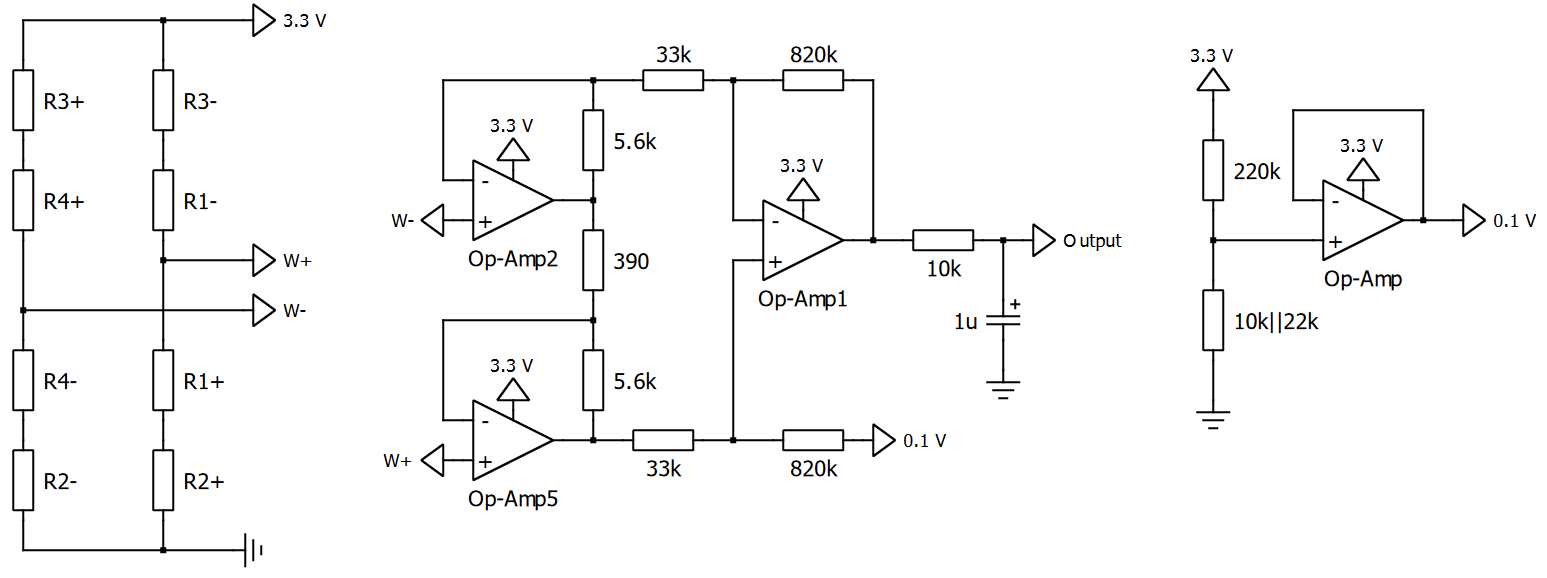
\includegraphics[scale=0.3]{schematic.png}
	\caption{Hardware schematic.}
	\label{fig:schematic}
\end{figure}

\begin{figure}[!ht]
	\centering
	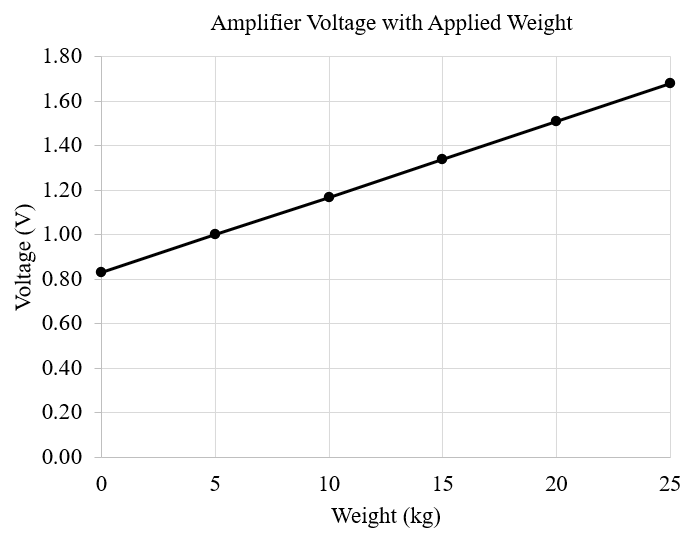
\includegraphics[scale=0.38]{simulation.png}
	\caption{Hardware simulation results.}
	\label{fig:simulation}
\end{figure}



